\documentclass{article}
\usepackage{booktabs}
\usepackage{amsmath}
\usepackage{graphicx}
\usepackage{caption}
\usepackage{listings}
\usepackage{xcolor}
\usepackage{pxfonts}
\lstset{
  basicstyle=\ttfamily,
  columns=fullflexible,
  breaklines=true,
  postbreak=\raisebox{0ex}[0ex][0ex]{\color{red}$\hookrightarrow$\space}
}
\title{Homework}
\author{Zhijiia Chen}
\begin{document}
\maketitle
\section{HW1}

\paragraph{4.} Describe the workflow of watching a video station, specifying each step what the application layer’s protocols are used.

Suppose we access the video station through its website.

1. Use DNS protocol to resolve the domain of the video station

2. Use HTTP/HTTPS protocol to request TV content web pages

\noindent \paragraph{5.} Hash table:

Can I use hash key as an id? Specify the reason.

No. A hash function is a multiple-to-one mapping which means for a certain item, its hash value is not unique, while an id by its definition should be unique.

How to find the difference between two list of strings?

For each pair of corresponding strings in the two list, first compare their hash values, if their hash values are different, then they are different. Otherwise, since having the same hash value does not guarantee the two strings are identical, we still need to compare the two strings character by character.

How to handle the duplication of the hash code?

We can do rehash by using new hash functions. We can also use open hash addressing such as chaining, linear probing.

How to deal with an shared hash table being used on the web server?

1. When updating the harsh table, lock the table. Each time, there are only one request can update the table. Save space because we only need to keep one copy of the table. But waste time, other requests need to wait.

2. Each request works on its own copy of the table, as long as they are not updating the same entry, the changes distributed among those copies can be merged. But if there multiple requests are updating the same entry, a lock is still needed. It saves time but wastes space.

\section{HW2}

\paragraph{1.} What are the transport layer protocols used for live video, file transfer, DNS and email, respectively?

\noindent \textbf{answer}: UDP, TCP, UDP, TCP

\paragraph{2.} Suppose we are using the TCP reno implementation.

\textbf{Phase 1}: slow start. Double the window size after each successful transmission. Window size of 1st transmission: 1 MSS. Window size of 2nd transmission: 2MSS. Window size of 3rd transmission: 4 MSS. Window size of 4th transmission: 8 MSS. A timeout occurs, set ssthreshold to half of current window size, i.e., 4 MSS, and set window size to 1. Window size of 5th transmission: 1 MSS. Window size of 6th transmission: 2 MSS. Window size of 7th transmission: 4 MSS. The window size reaches the ssthreshold, leaving Phase 1 and entering phase 2.

\textbf{Phase 2}: congestion avoidance. Increase windwo size by one after each successful transmission. Window size of 8th transmission: 5 MSS.

So by the end of 8th transmission, the congestion windows size is 5 MSS.

\paragraph{3.}

Source IP field: 1001100100010010 0000100001101001

Destination IP field: 1010101100000010 0000111000001010

Protocol field: 00010001

The length of the pseudoheader is 12 bytes.

The length of the head is 8 bytes.

The length of the payload after padding is 8 bytes.

UDP total length (28 bytes) field: 0000000000011100

Source port field: 0000010000111111

Destination port field: 0000000000001101

Data field: 0101010001000101 0101001101010100 0100100101001110 0100011100000000

Add up every 16 bits of the above fields (pad zeros if the length of a field is not the multiple of 16) with overflow bit wrapped around, we get 1001011011101001. Then we take the 1's complement of the sum to get the checksum 0110100100010110.

\paragraph{4.} I run the nmap command "nmap -sP 192.168.56.1-128" in my linux virtual machine and got the output copied below. I have two linux VMs running on my Mac and they are attached to a virtual subnet. So the command probes the available hosts in the network. In the above output, host 192.168.56.1 is my Mac, and host 192.168.56.101 and host 192.168.56.102 are the VMs.

Starting Nmap 7.60 ( https://nmap.org ) at 2018-10-24 12:01 EDT

Nmap scan report for 192.168.56.1

Host is up (0.00051s latency).

Nmap scan report for zhijia-VirtualBox (192.168.56.101)

Host is up (0.000086s latency).

Nmap scan report for 192.168.56.102

Host is up (0.00077s latency).

Nmap done: 128 IP addresses (3 hosts up) scanned in 17.16 seconds

\section{HW3}

\paragraph{1.} Assign a letter to each node as shown in Fig.~\ref{fig:topo}.
\begin{figure}
    \centering
    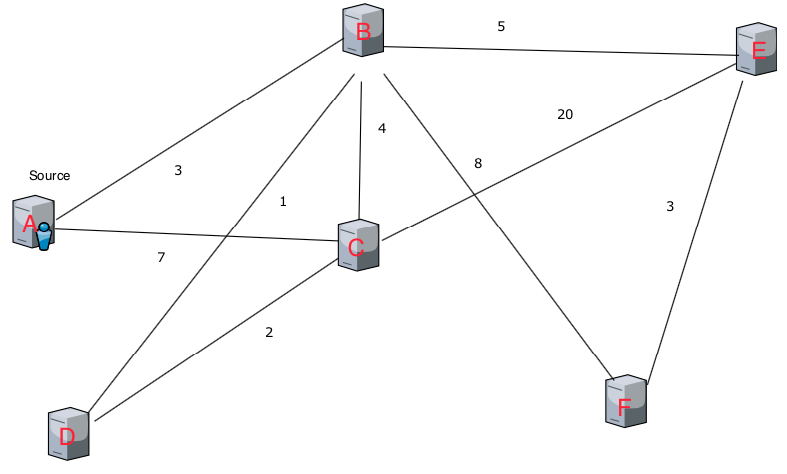
\includegraphics[width=\linewidth]{fig/topo.png}
    \caption{network topology
    } \label{fig:topo}
\end{figure}
Define the following notation:

\begin{itemize}
    \item $d(v)$: cost of the least-cost path from the source node to destination $v$ as of this iteration of the algorithm.
    \item $d_x(y)$ current minimum cost from node x to node y.
    \item $c(x, y)$ cost from x to directly attached neighbor y.
    \item $p(v)$: previous node (neighbor of $v$) along the current least-cost path from the source to $v$.
    \item $N$: all the nodes.
    \item $N'$: subset of nodes; $v$ is in $N'$ if the least-cost path from the source to $v$ is definitively known.
\end{itemize}

\textbf{Link-State (Dijkstra algorithm)}: 

\begin{lstlisting}[mathescape=true]
    N' = {A}
    for all nodes v
        if v is a neighbor of A then
            d(v) = c(A, v)
        else 
            d(v) = $\infty$
    loop
        find w not in N' such that d(w) is a minimum
        add w to N'
        update d(V) for each neighbor v of w and not in N':
            d(v) = min(d(v), d(w) + c(w, v))
    until N' = N
\end{lstlisting}

Table~\ref{tab:dijkstra} shows the result of each step using Dijkstra to find the shortest paths.
\begin{table}[h!]
    \begin{center}
      \caption{Find shortest path using Dijkstra algorithm.}
      \label{tab:dijkstra}
      \begin{tabular}{c|c|c|c|c|c|c|c} % <-- Alignments: 1st column left, 2nd middle and 3rd right, with vertical lines in between
        \toprule
        \textbf{Picked node}& \textbf{N'}& \textbf{A}&\textbf{B}&\textbf{C}&\textbf{D}&\textbf{E}&\textbf{F}\\
        \hline
        A&{A}&-&A, 3&A, 7&$\infty$&$\infty$&$\infty$\\
        \hline
        B&{A, B}&&-&A, 7&B, 4&B, 8&B, 11\\
        \hline
        D&{A, B, D}&&&D, 6&-&B, 8&B, 11\\
        \hline
        C&{A, B, C, D}&&&-&&B, 8&B, 11\\
        \hline
        E&{A, B, C, D, E}&&&&&-&B, 11\\
        \hline
        F&{A, B, C, D, E, F}&&&&&&-\\
        \bottomrule
      \end{tabular}
    \end{center}
  \end{table}

\textbf{Distance-Vector}:

At each node x:
\begin{lstlisting}[mathescape=true]
    for all destinations y in N:
        $d_x$(y) = c(x, y) /* if y is not a neighbor, then c(x, y) = $\infty$ */
    for each neighbor w
        $d_w$(y) = $\infty$ for all destinations y in N
    for each neighbor w
        send distance vector $D_x$ = [$d_x$(y): y in N] to w
    loop
        wait (until sense a link cost change to some neighbor w or until receive a a distance vector from some neighbor w)
        for each y in N:
            $d_x$(y) = $min_v${c(x, v) + d_v(y)}
        if $d_x$(y) changed for any destination y
            send distance vector $D_x$ = [$d_x$(y): y in N] to all neighbors
    forever
\end{lstlisting}

Table~\ref{tab:initial-vector} shows the initial distance vector that broadcasted by each node. After one round of broadcasting, each node gets the shortest path to all other nodes. Table~\ref{tab:final-vector} shows the stablized distance vectors that broadcasted by each node.

\begin{table}[h!]
    \begin{center}
        \caption{Initial distance vectors}
        \label{tab:initial-vector}
        \begin{tabular}{c|c|c|c|c|c|c} % <-- Alignments: 1st column left, 2nd middle and 3rd right, with vertical lines in between
        \toprule
        \textbf{broadcasting node}& \textbf{A}&\textbf{B}&\textbf{C}&\textbf{D}&\textbf{E}&\textbf{F}\\
        \hline
        \textbf{A}&0&3&7&$\infty$&$\infty$&$\infty$\\
        \hline
        \textbf{B}&3&0&4&1&5&8\\
        \hline
        \textbf{C}&7&4&0&2&20&$\infty$\\
        \hline
        \textbf{D}&$\infty$&1&2&0&$\infty$&$\infty$\\
        \hline
        \textbf{E}&$\infty$&5&20&$\infty$&0&3\\
        \hline
        \textbf{F}&$\infty$&8&$\infty$&$\infty$&3&0\\
        \bottomrule
        \end{tabular}
    \end{center}
\end{table}

\begin{table}[h!]
    \begin{center}
        \caption{Final distance vectors}
        \label{tab:final-vector}
        \begin{tabular}{c|c|c|c|c|c|c} % <-- Alignments: 1st column left, 2nd middle and 3rd right, with vertical lines in between
        \toprule
        \textbf{broadcasting node}& \textbf{A}&\textbf{B}&\textbf{C}&\textbf{D}&\textbf{E}&\textbf{F}\\
        \hline
        \textbf{A}&0&3&7&4&8&11\\
        \hline
        \textbf{B}&3&0&4&1&5&8\\
        \hline
        \textbf{C}&7&4&0&2&9&12\\
        \hline
        \textbf{D}&4&1&2&0&6&9\\
        \hline
        \textbf{E}&8&5&20&6&0&3\\
        \hline
        \textbf{F}&11&8&12&9&3&0\\
        \bottomrule
        \end{tabular}
    \end{center}
\end{table}

\paragraph{2.}

\begin{enumerate}
    \item DNS lookup using UDP.
    \item Initiate a TCP connection with the server.
    \item Request the webpage using HTTP/HTTTPS protocol.
\end{enumerate}

\paragraph{3.}

\begin{enumerate}
    \item setup VPN service in the destination node, create user credentials such as account and password.
    \item Get the IP address of the VPN server and requests accounts and password.
    \item Use platform utilities to open VPN connection to the server.
\end{enumerate}

\section{HW4}

\paragraph{1.} Table ~\ref{tab:transferred} shows the data with even parity check bits to be transferred.

\begin{table}[h!]
    \begin{center}
      \caption{data to be transferred}
      \label{tab:transferred}
      \begin{tabular}{c|c|c} % <-- Alignments: 1st column left, 2nd middle and 3rd right, with vertical lines in between
        \toprule
        & \textbf{Raw Data} & \textbf{Check}\\
        \hline
        &1001&0\\
        \hline
        &1100&0\\
        \hline
        &0110&0\\
        \hline
        &0111&1\\
        \hline
        \textbf{Check}&0100&0\\
        \bottomrule
      \end{tabular}
    \end{center}
  \end{table}

  Table ~\ref{tab:corrected} shows the corrected data with even parity check bits. We suppose that the CRC is intact. We first check each column and we see that the first column does not match the parity bit, so we know there must be some error in the first column. We then check each row, and we see find that the second row also do not match the parity bit. Thus we know that it's very likely that the first column of the second row is incorrect, and we correct the bit to 1. 
  \begin{table}[h!]
    \begin{center}
      \caption{corrected data with CRC check}
      \label{tab:corrected}
      \begin{tabular}{c|c|c} % <-- Alignments: 1st column left, 2nd middle and 3rd right, with vertical lines in between
        \toprule
        & \textbf{Raw Data} & \textbf{Check}\\
        \hline
        &1001&0\\
        \hline
        &1100&0\\
        \hline
        &0110&0\\
        \hline
        &0111&1\\
        \hline
        \textbf{Check}&0100&0\\
        \bottomrule
      \end{tabular}
    \end{center}
  \end{table}

\paragraph{2. } I could not used the given code to recover data correctly, so I used the code in the slides instead.

Code for user1:

 1,  1,  1, -1,  1, -1, -1, -1

Code for user2:

 1, -1,  1,  1,  1, -1,  1,  1

User1's data: -1, -1

User2's data: 1, -1

First expand user data by repeating each bit for 8 times. 

Expanded data of user1:

-1, -1, -1, -1, -1, -1, -1, -1,

-1, -1, -1, -1, -1, -1, -1, -1

Expanded data of user1:

 1,  1,  1,  1,  1,  1,  1,  1, 

-1, -1, -1, -1, -1, -1, -1, -1

Multiply user data with the corresponding code.

Signal sent out by user1:

 1, -1, -1,  1, -1,  1,  1,  1,

-1, -1, -1,  1, -1,  1,  1,  1

Signal sent out by user2:

 1, -1,  1,  1,  1, -1,  1,  1

-1,  1, -1, -1, -1,  1, -1, -1

Data wave form received by both user1 and user2:

 0, -2,  0,  2,  0,  0,  2,  2,

-2,  0, -2,  0, -2,  2,  0,  0

To restore data, receiver multiplies each block of data with corresponding code and get the average.

The multiplication output of receiver1:

 0, -2,  0, -2,  0,  0, -2, -2

-2,  0, -2,  0, -2, -2,  0,  0

And average of each data block: -1, -1

The multiplication output of receiver2:

 0,  2,  0,  2,  0,  0,  2,  2,

-2,  0, -2,  0, -2, -2,  0,  0

And average of each data block: 1, -1

\paragraph{3.} In CSMA/CD data packets collide. In CSMA/CA only control packets collide.  When CSMA/CD was used in wireless transmission, especially in an open Wifi spectrum, there are very high chances that the packets can collide very often resulting in lot of re-transmissions and ultimately ruining the bandwidth. So CSMA/CA is more scalable for multi user open air communication.

\paragraph{4.} Triangle routing is a routing scheme that supports mobile IP. For example, when a correspondent node wants to connects to a mobile node that is currently outside of home agent but with some foreign agent, the correspondent nodes does not need be worry about (or even aware of) this problem, and sends all packets to the mobile node's home address. Then the home agent then tunnels them to mobile node's foreign address, and the mobile node sends its packets directly to the correspondent node.

Pros: provides mobility, transparent to the correspondent nodes

Cons: expensive, correspondent's packets need to go through unnecessary routes.

\section{HW5}

\paragraph{1.} Shown in the Fig.\ref{fig:openssl}.

\noindent \paragraph{2.} Shown in the Fig.\ref{fig:ssh-keygen}.

\noindent \paragraph{3.} Shown in the Fig.\ref{fig:keytool}.

\noindent \paragraph{4.} Shown in the Fig.\ref{fig:CSR}.

\noindent \paragraph{5.} Shown in the Fig.\ref{fig:certificate}.

\noindent \paragraph{6.} Shown in the Fig.\ref{fig:verify}.

\begin{figure}
    \centering
    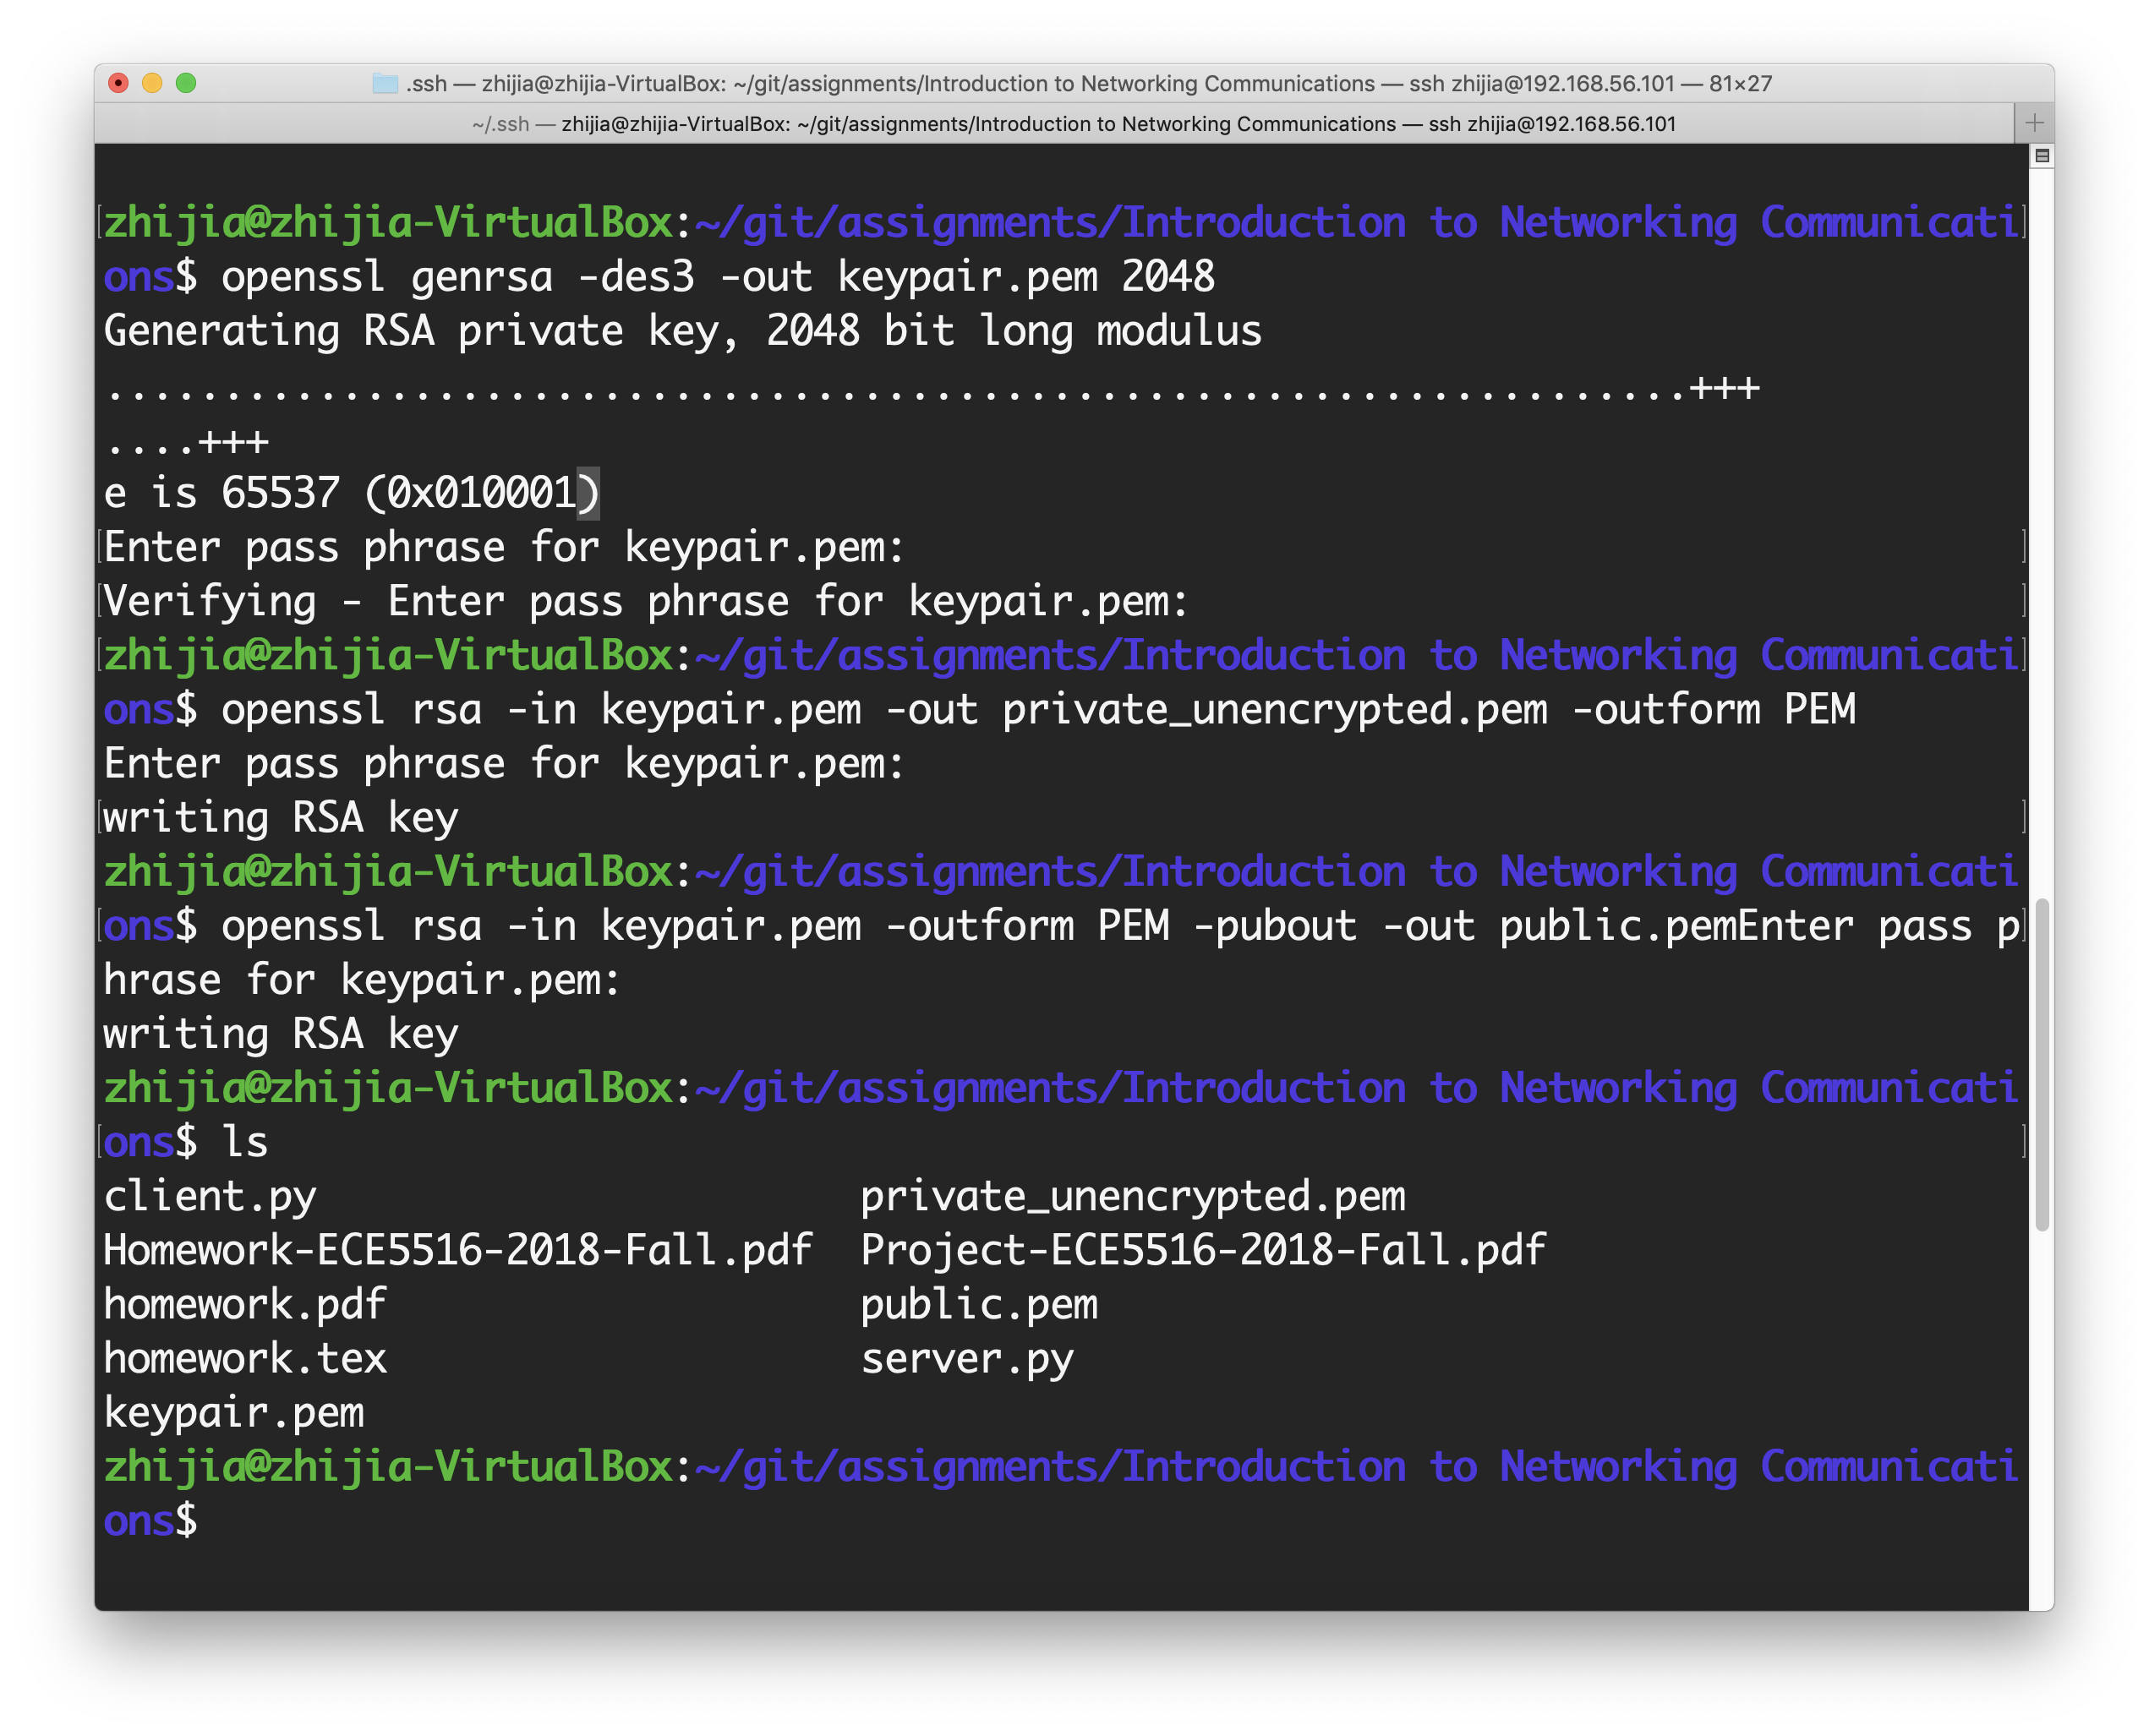
\includegraphics[width=\linewidth]{fig/openssl.png}
    \caption{Use openssl to create private key and public key.
    } \label{fig:openssl}
\end{figure}

\begin{figure}
    \centering
    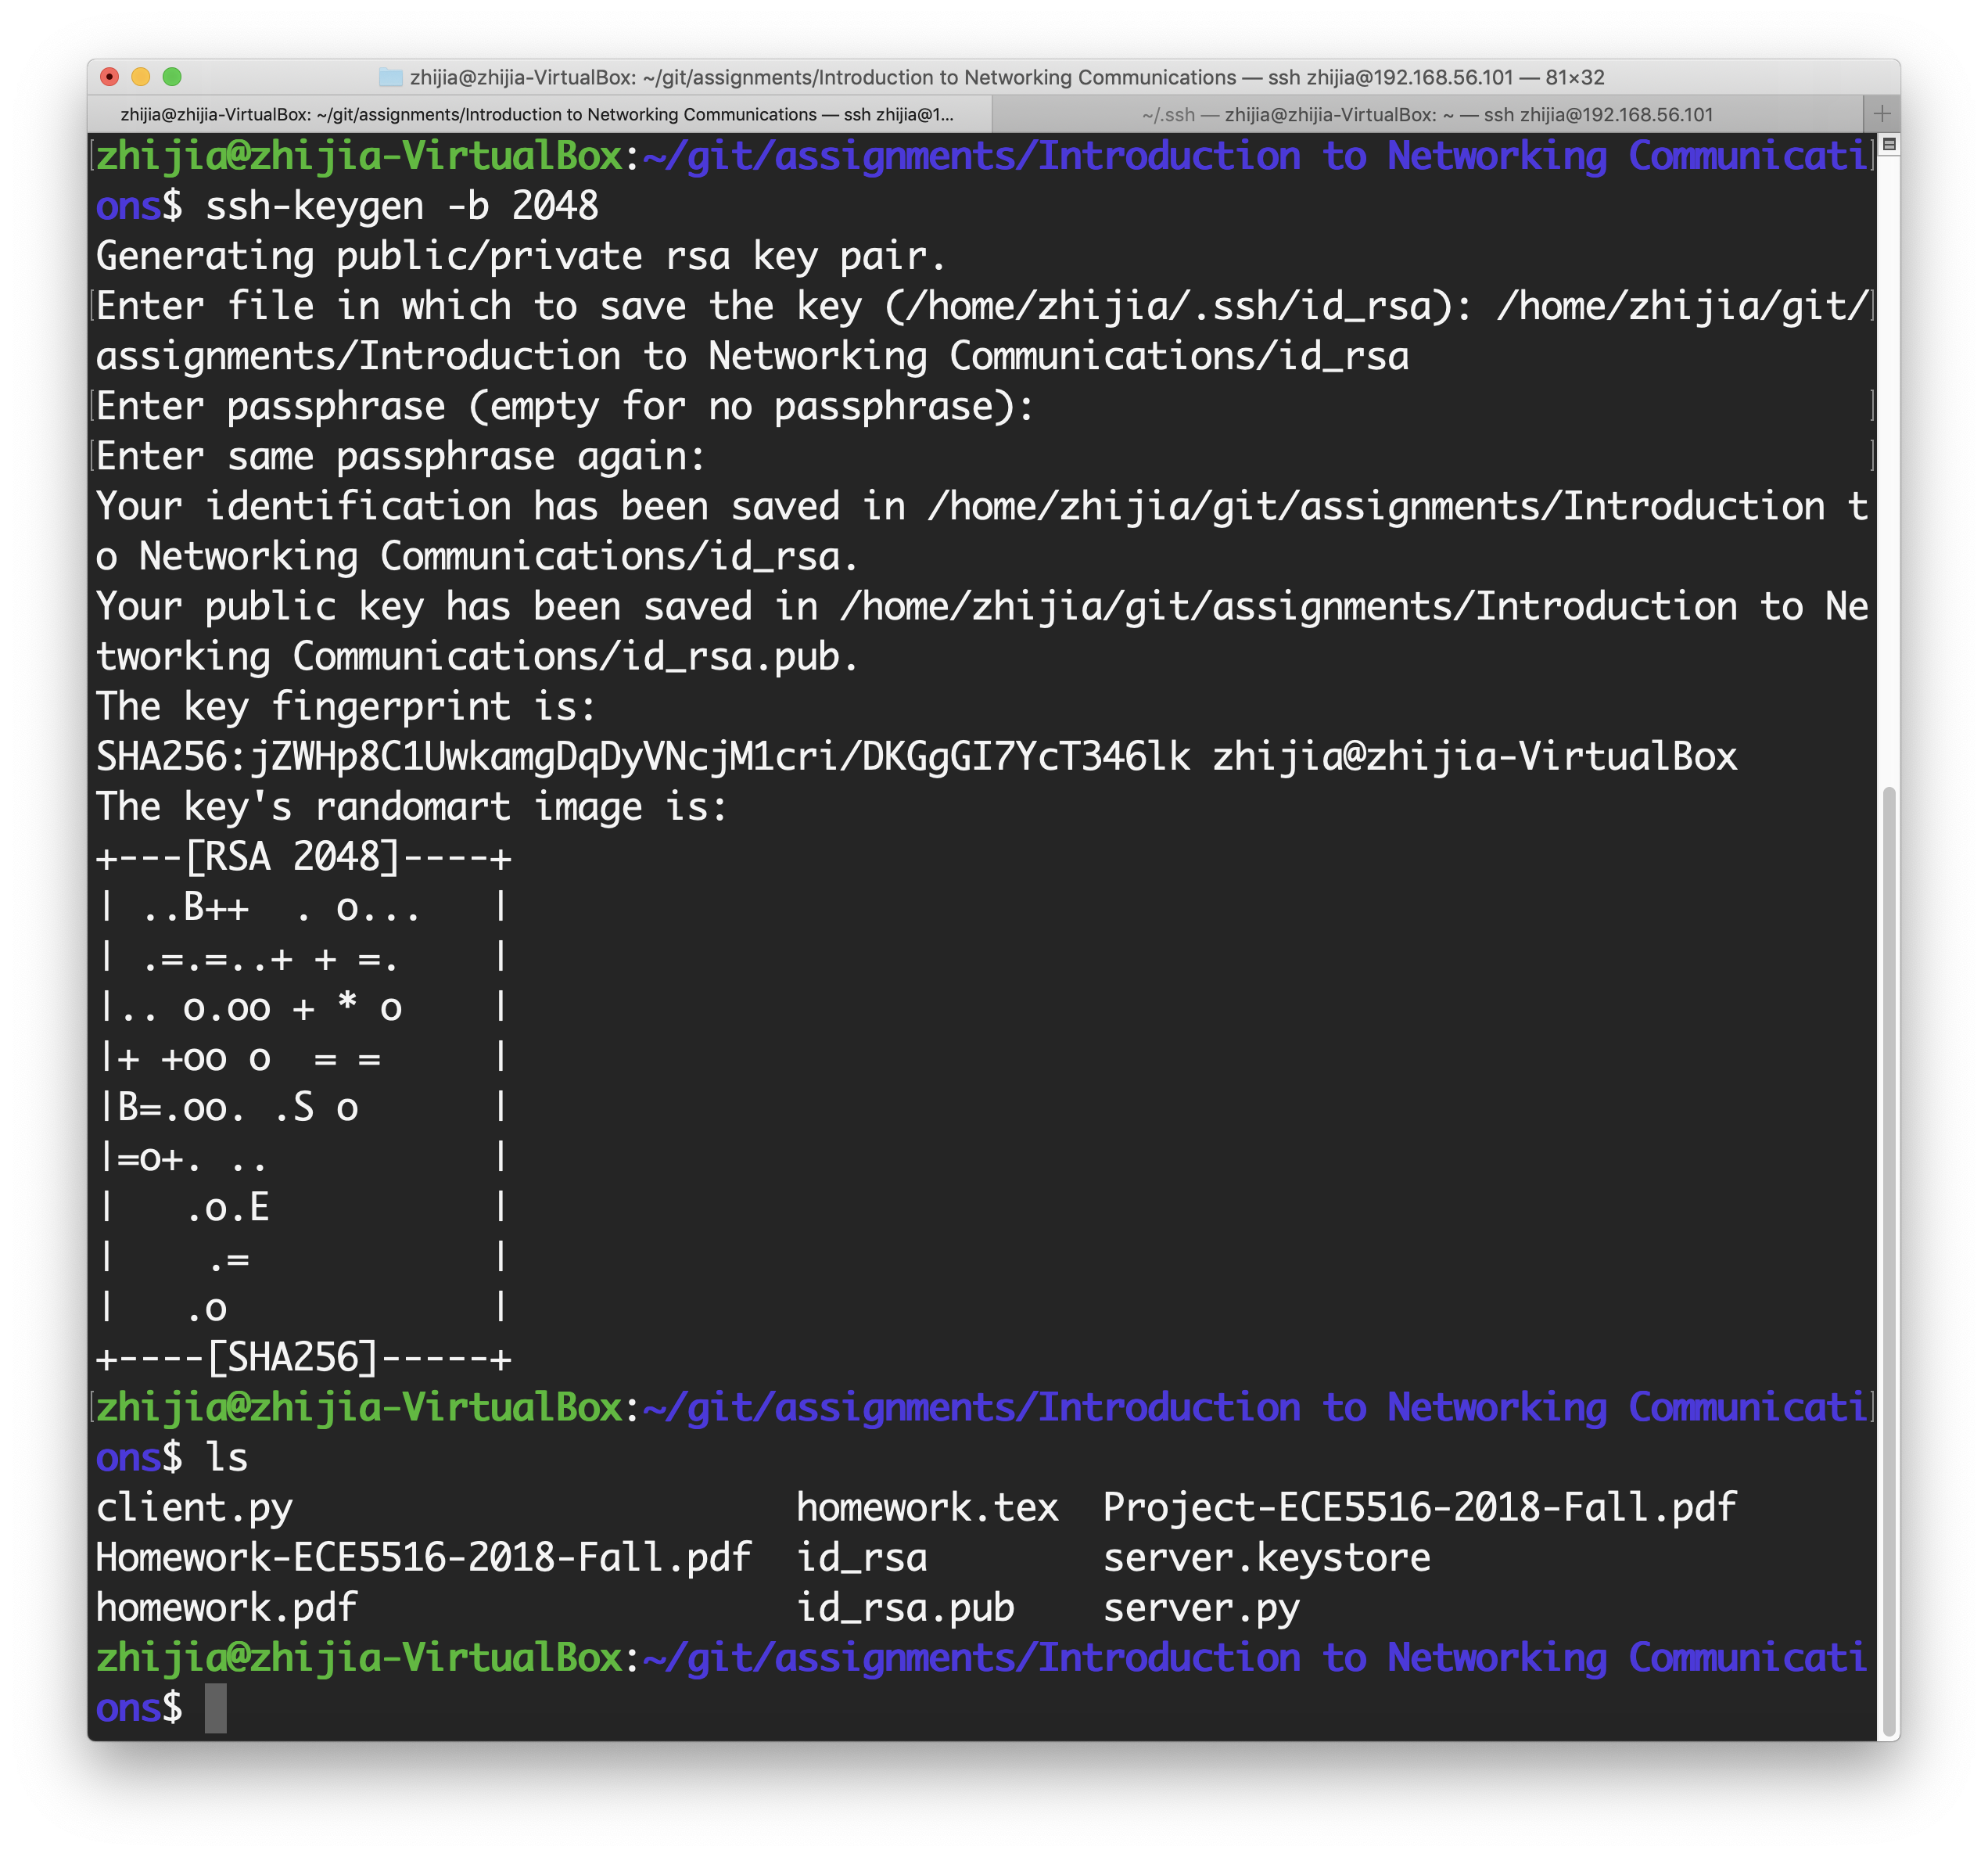
\includegraphics[width=\linewidth]{fig/ssh-keygen.png}
    \caption{Use ssh-keygen to create private key and public key.
    } \label{fig:ssh-keygen}
\end{figure}

\begin{figure}
    \centering
    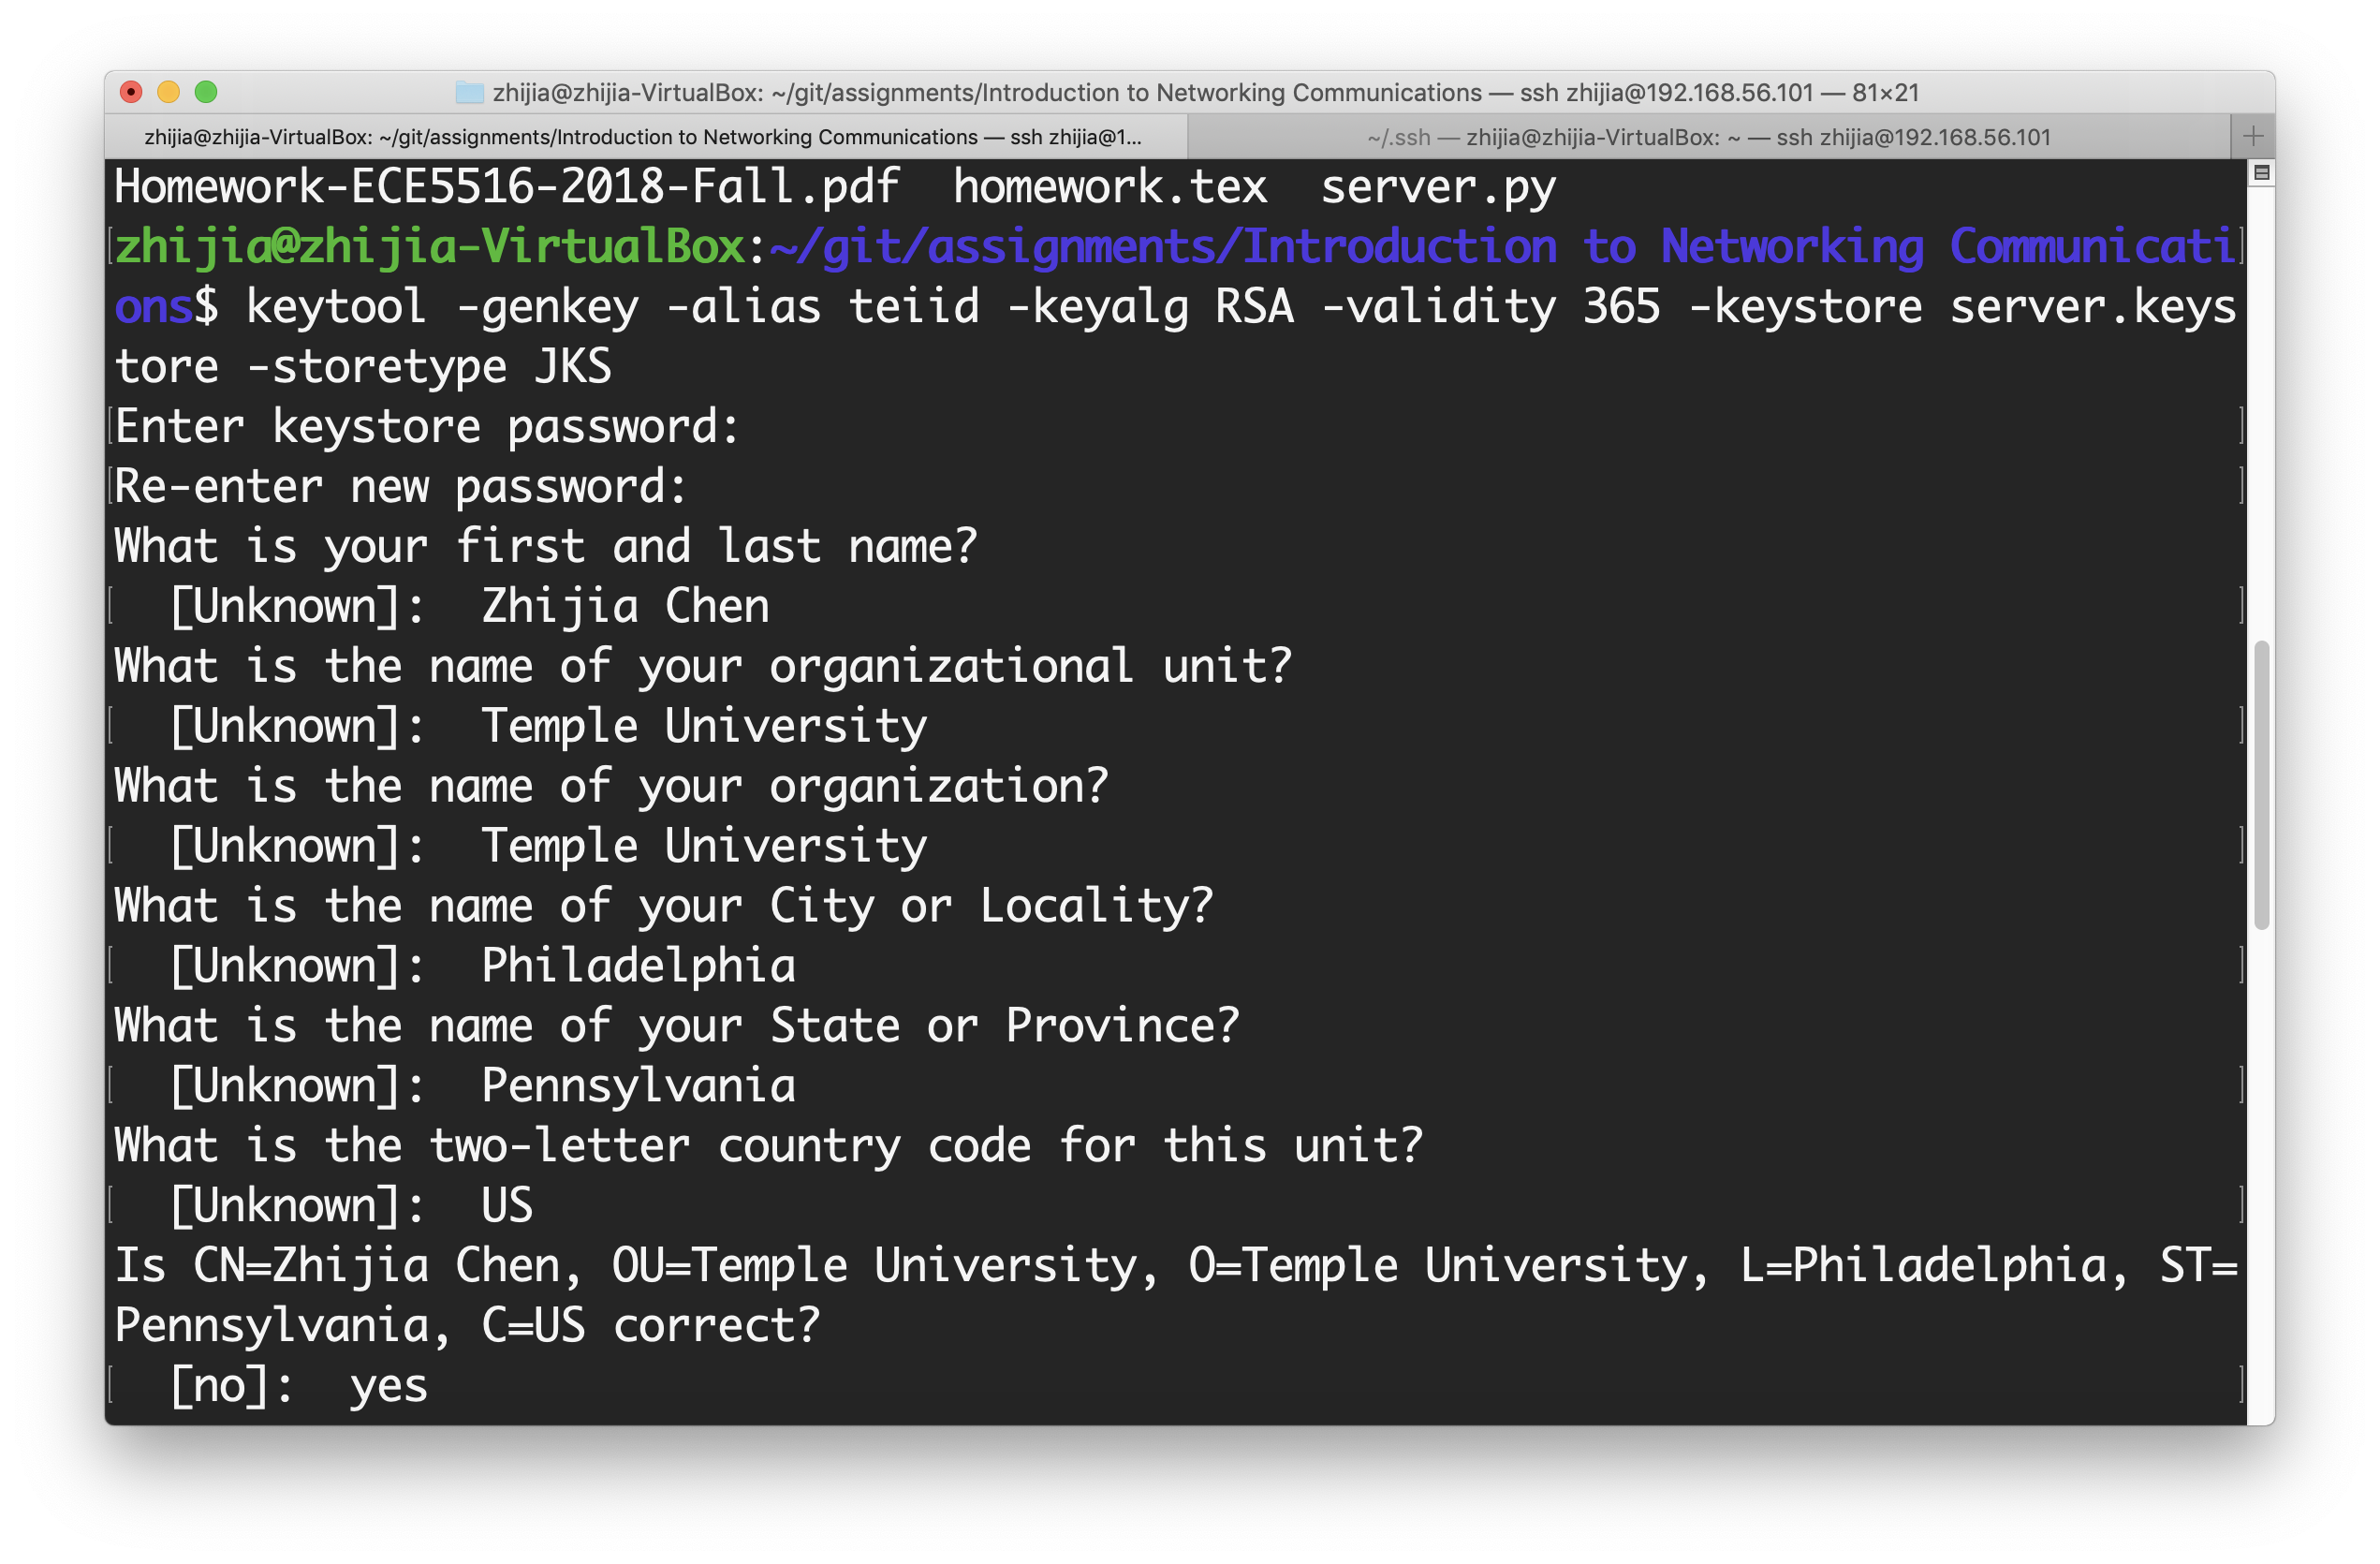
\includegraphics[width=\linewidth]{fig/keytool.png}
    \caption{Use keytool to create private key and public key pair in a keystore.
    } \label{fig:keytool}
\end{figure}

\begin{figure}
    \centering
    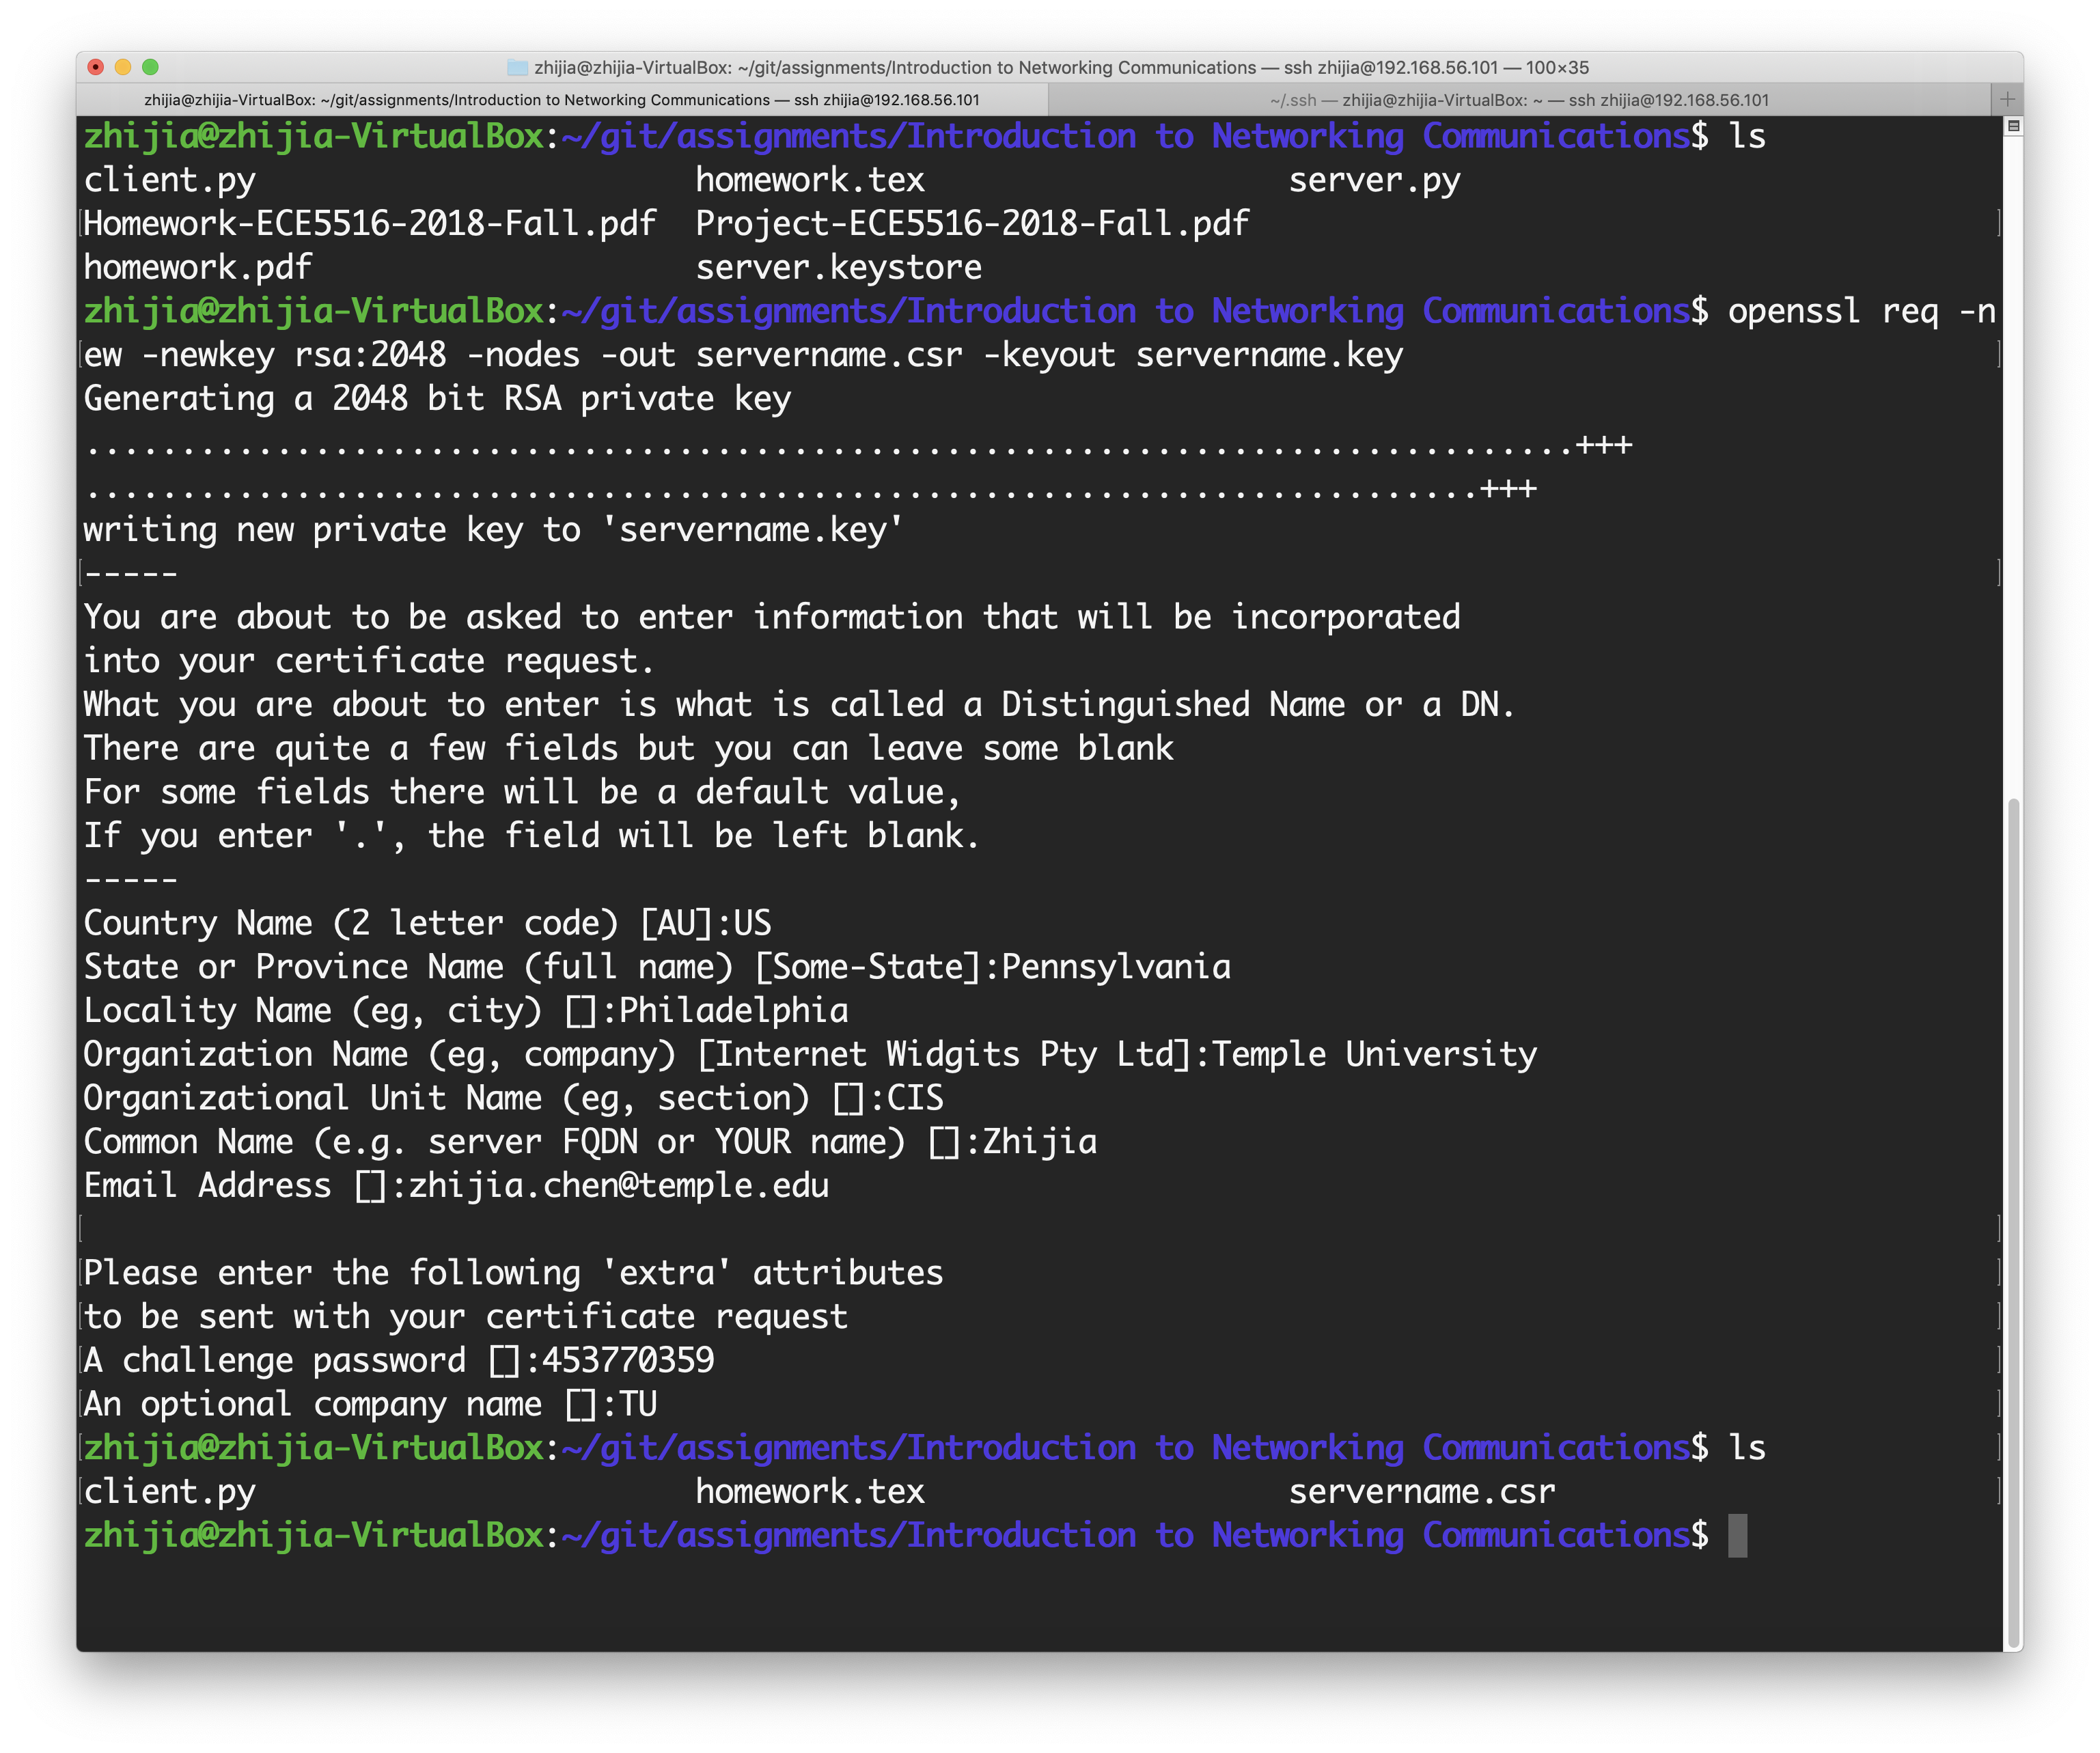
\includegraphics[width=\linewidth]{fig/CSR.png}
    \caption{Use openssl to create a private key and CSR.
    } \label{fig:CSR}
\end{figure}

\begin{figure}
    \centering
    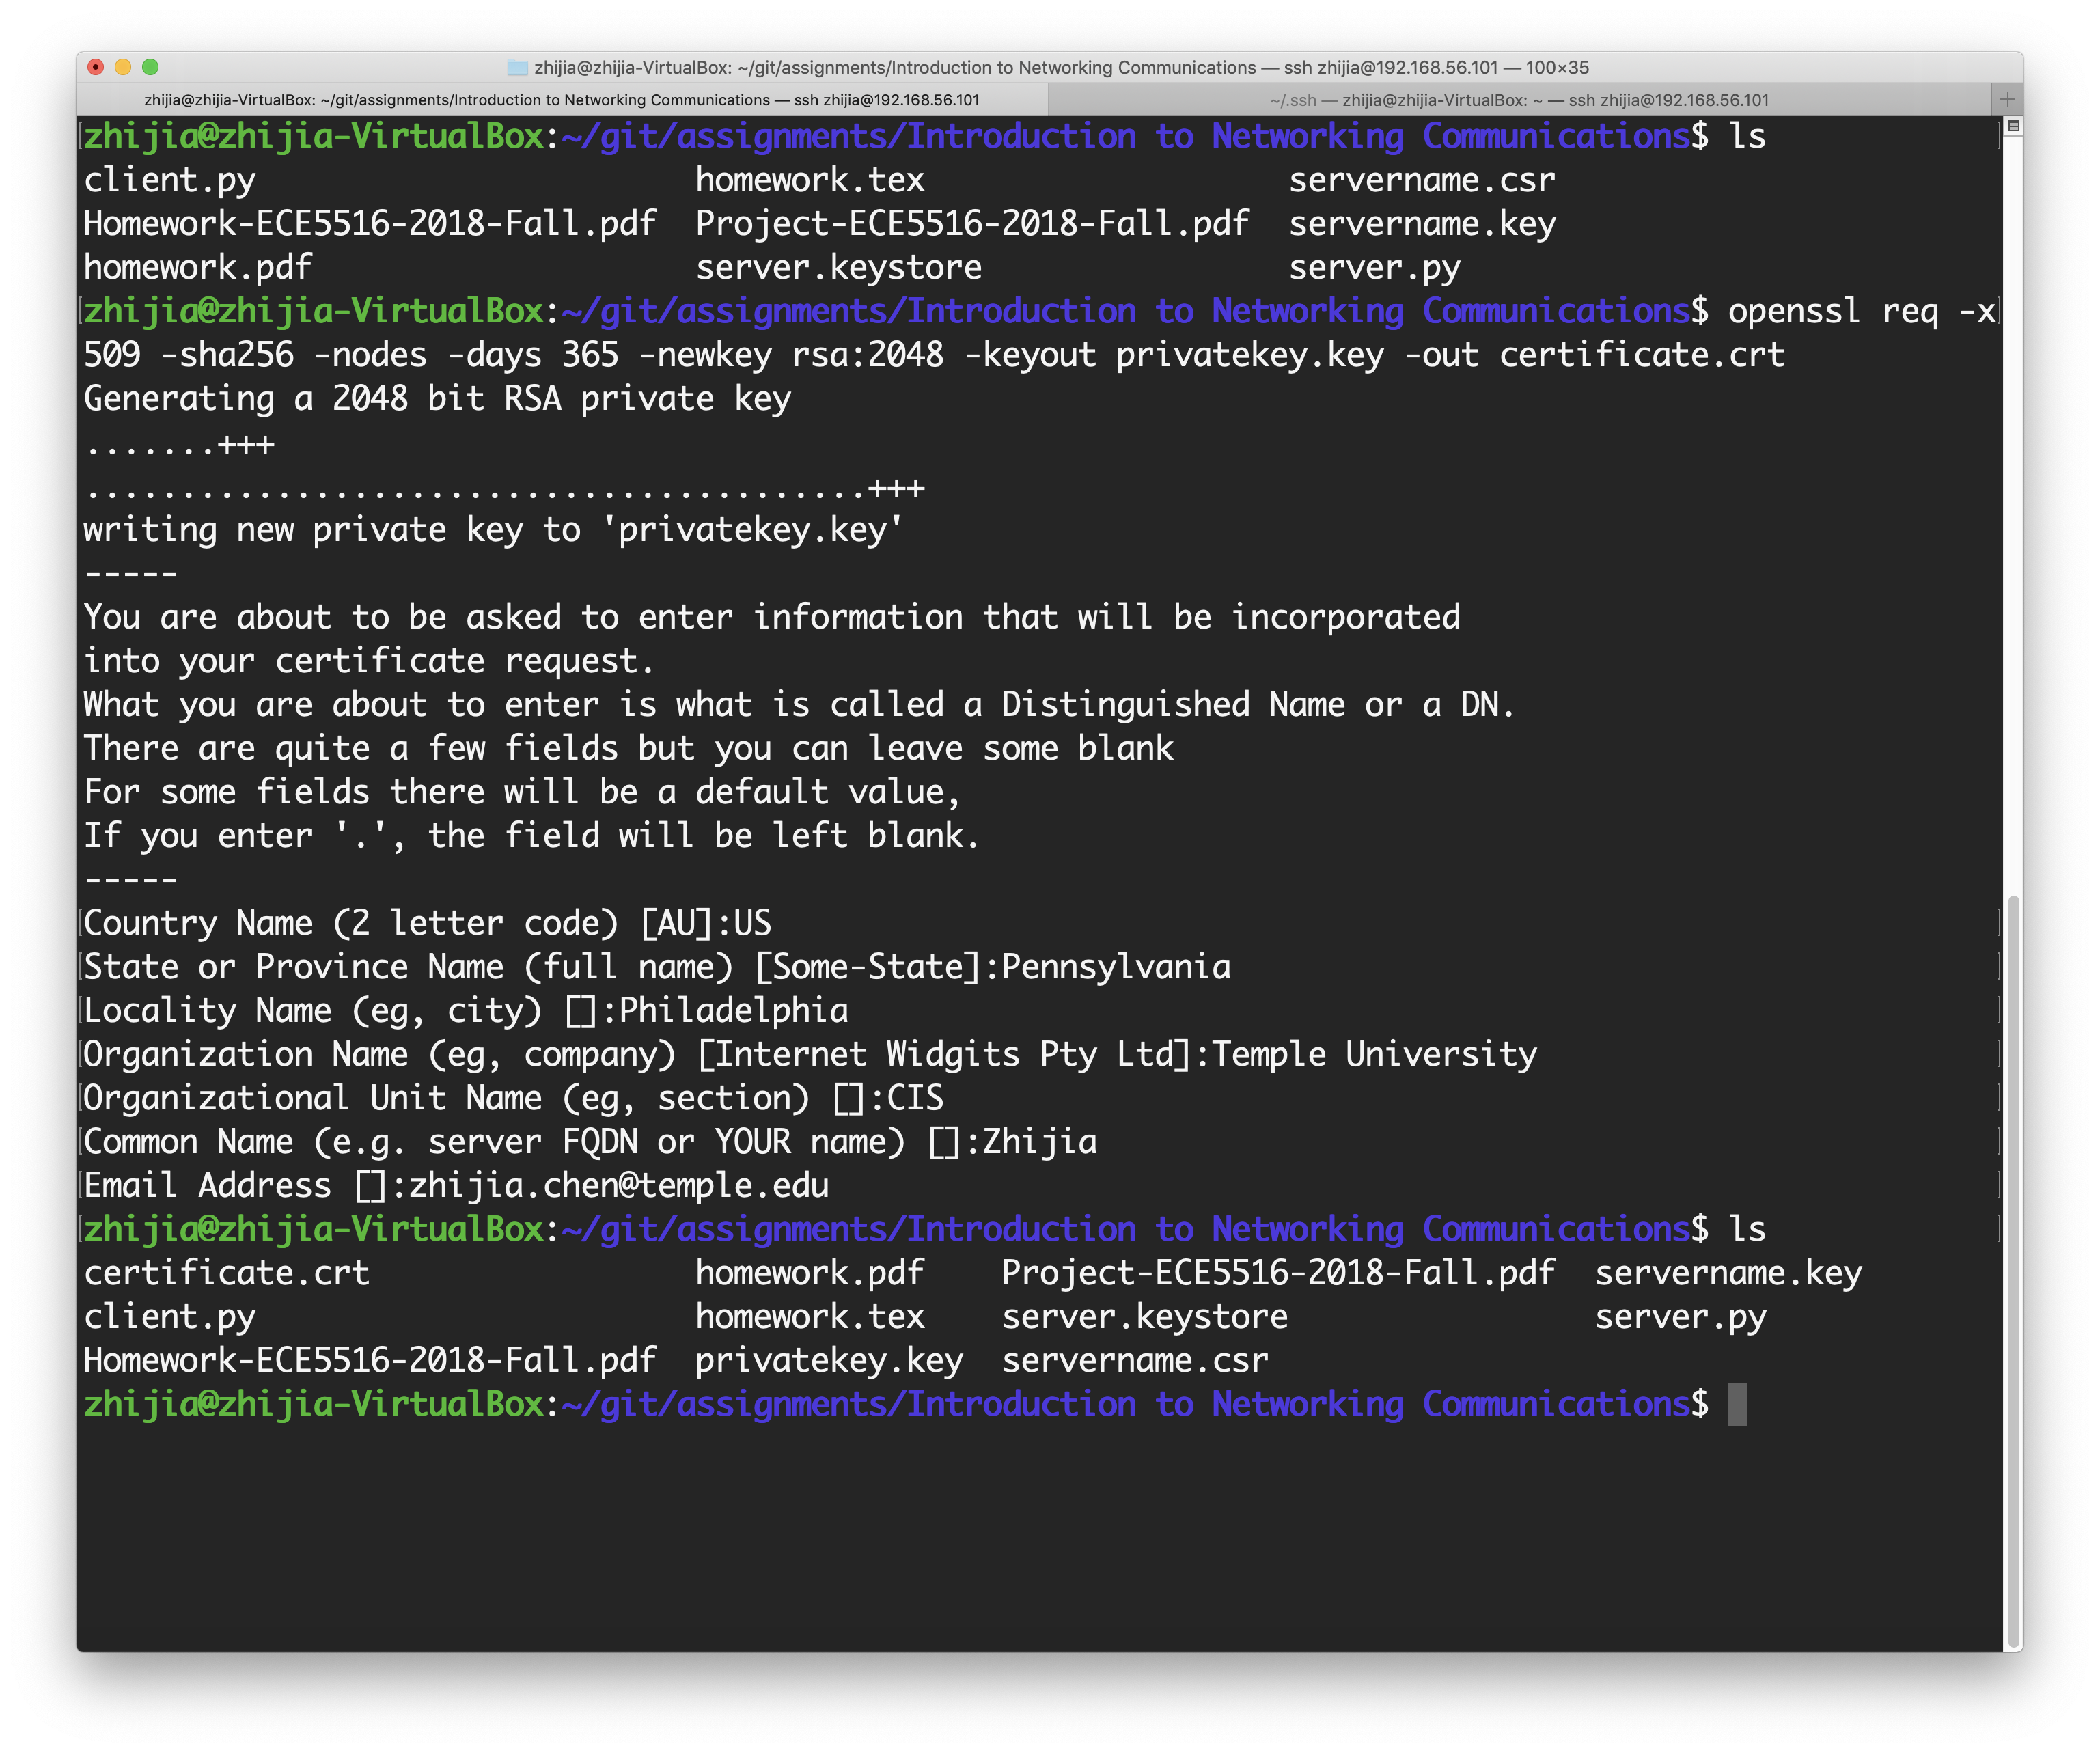
\includegraphics[width=\linewidth]{fig/certificate.png}
    \caption{Use openssl to create a private key and a certificate.
    } \label{fig:certificate}
\end{figure}

\begin{figure}
    \centering
    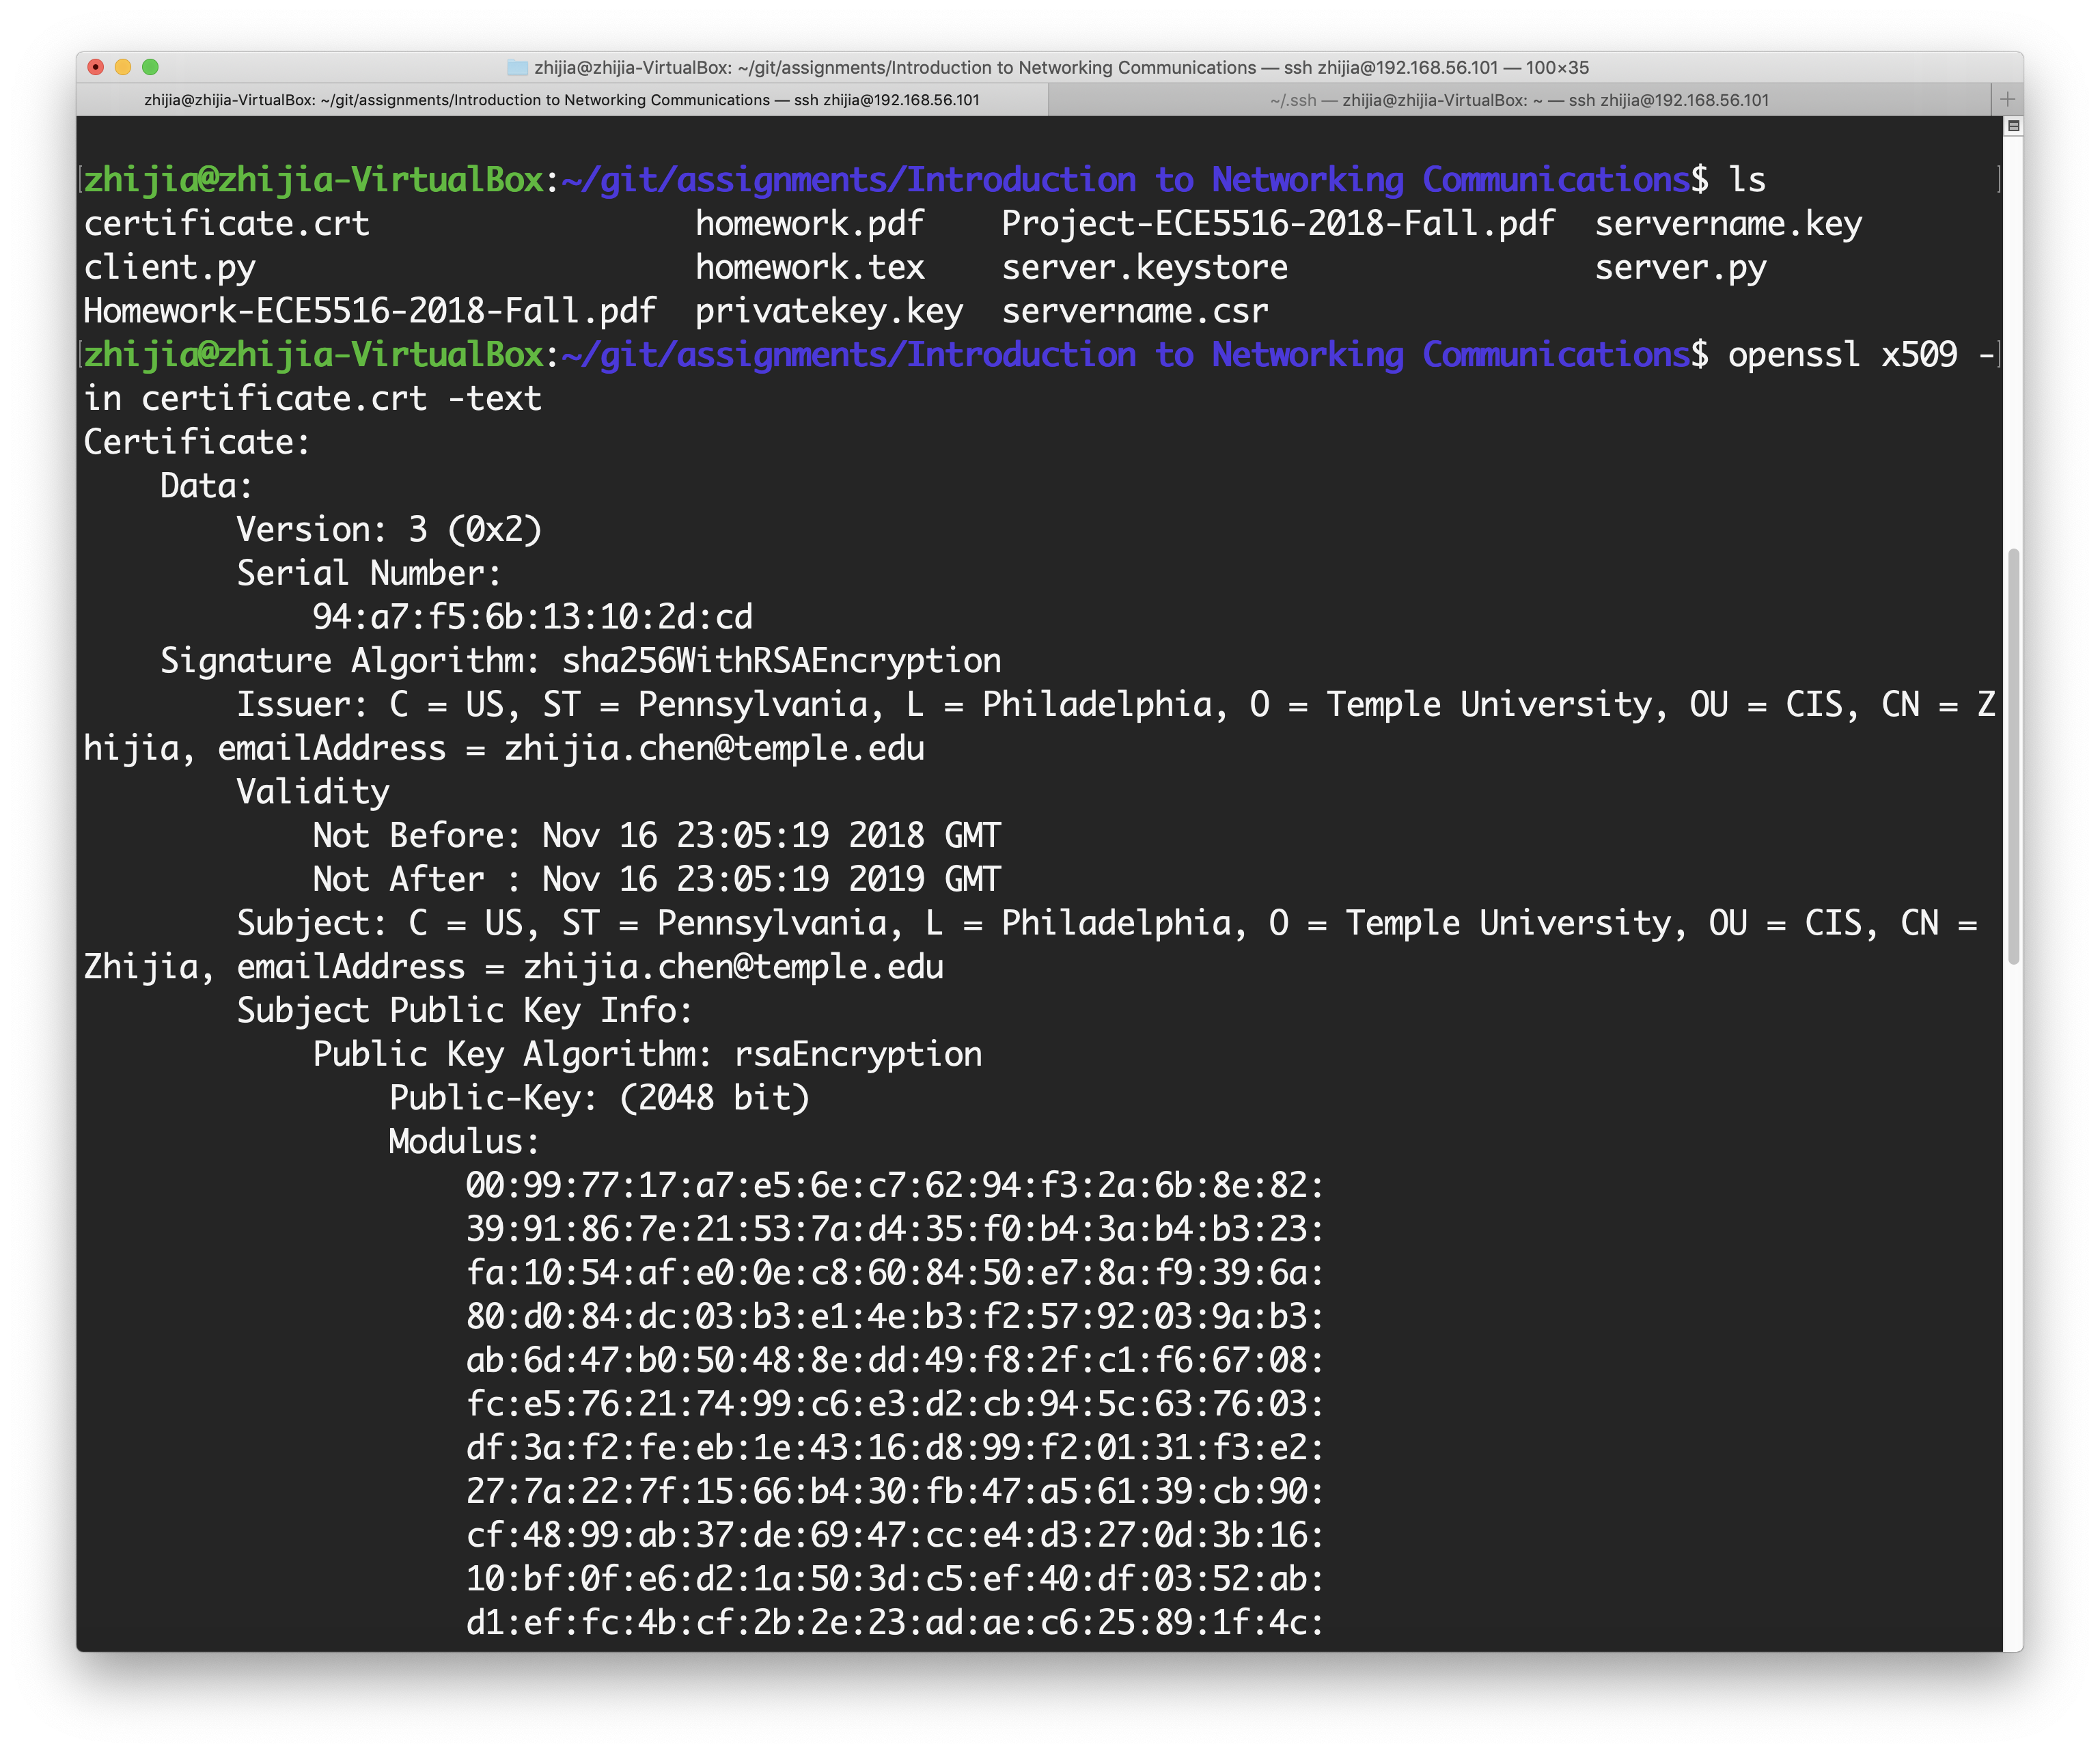
\includegraphics[width=\linewidth]{fig/verify.png}
    \caption{Use openssl to verify a certificate.
    } \label{fig:verify}
\end{figure}
\end{document}
